% \chapter{
% 	۱)بررسی انواع مدل‌های ارائه شده برای دیتابیس‌ها و مزایا و معایب آن‌ها نسبت به مدل رابطه‌ای
% }

\section*{\centering ۱) بررسی انواع مدل‌های ارائه شده برای دیتابیس‌ها و مزایا و معایب آن‌ها نسبت به مدل رابطه‌ای
}



‌از انواع مختلف مدل‌های ارائه شده برای ساخت دیتابیس می‌توان به مدل 
$Hierarchical$
،‌
$Network$
،
$Relational$
،
$Object Oriented $
یا
$Object Relational$
اشاره کرد که آن‌ها را، با تمرکز بر مدل رابطه‌ای، بررسی خواهیم کرد.

در مدل 
$Hierarchical$
یا همان مدل درختی، که با نام «مدل سلسله مراتبی» نیز شناخته می‌شود،  همان طور که از نام این مدل مشخص است، در آن داده‌ها در ساختمان‌داده‌ای مشابه  درخت ذخیره می‌شوند.
در ریشه که بالاترین سطح درخت است، 
$Root Node$
قرار دارد.
هر یک از گره‌هایی که در سطح بعدی درخت قرار دارد، شامل یک نمونه از داده‌هایی‌ست که قصد ذخیره سازی آن را داریم.
برای مثال اگر قصد ذخیره سازی داده‌های مربوط به دانشجویان را داشته باشیم، فیلدهایی نظر 
$S_id$
،‌
$S_name$
،
$S_birthday$
و
$S_department$
در هر یک از گره‌های این سطح، ذخیره می‌شوند.

% \chapter{
% 	تعبیه همسایه تصادفی (اس ان ای)
% }
% اس ان ای با تبدیل فاصله‌ی اقلیدسی برای ابعاد بالا به یک تابع احتمال شرطی که نشان دهنده‌ی شباهت بین دو نقطه است کار خود را آغاز می‌کند.
% شباهت داده‌ی
% $x_i$
% با داده‌ی
% $x_j$
% به صورت تابع احتمال شرطی
% $p_{j|i}$
% نشان داده می‌شود.
% معنای این تابع احتمال این است که داده‌ی
% $x_i$
% داده‌ی
% $x_j$
% را به عنوان همسایه خود انتخاب کند که احتمال انتخاب داده‌ها به عنوان همسایه، یک توزیع گواسی به مرکزیت
% $x_i$
% می‌باشد.
% برای داده‌های نزدیک به
% $x_i$
% این احتمال نزدیک بالا و برای داده‌های دور از
% $x_i$
% این احتمال تقریبا بسیار کوچک است (اگر مقدار واریانس به خوبی انتخاب شود).
% فرمول این تابع به شکل زیر است:
% \begin{figure}[!h]
% 	\centering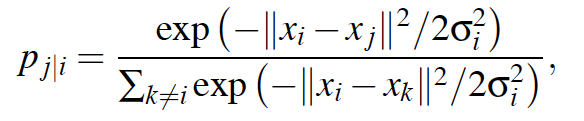
\includegraphics[scale=.3]{eq1}
% 	\caption{فرمول تابع احتمال شرطی}\label{fig.eq1}
% \end{figure}
% \\
% به دلیل اینکه ما به دنبال شباهت به صورت دوتایی داده‌ها هستیم مقدار
% $p_{i|i}$
% برابر با صفر در نظر گرفته می‌شود، همچنین نحوه به دست آوردن واریانس ($\sigma_i$) بعدا در این بخش توضیح داده می‌شود.
% \\
% اگر فرض کنیم که داده‌ی
% $x_i$
% به داده‌ی
% $y_i$
% و داده‌
% $y_i$
% به داده‌ی
% $y_j$
% نگاشت شده باشد، تابع احتمال شرطی دیگری مانند $p$ برای شباهت بین دو داده‌ی نگاشت داده شده به نام $q$ تعریف می‌کنیم که فرمول آن به شکل زیر است:
% \begin{figure}[!h]
% 	\centering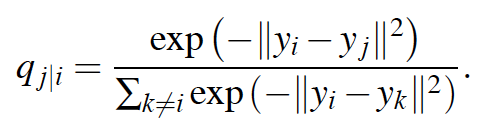
\includegraphics[scale=.3]{eq2}
% 	\caption{فرمول تابع احتمال شرطی برای داده‌های نگاشت داده شده}\label{fig.eq2}
% \end{figure}
% \\
% در ایت تابع نیز باز مقدار
% $q_{i|i}$
% برابر با صفر در نظر گرفته می‌شود و همچنین مقدار واریانس برابر با 
% $\frac{1}{\sqrt{2}}$
% در نظر گرفته شده است.
% \\
% در اس ان ای سعی می‌شود که تفاوت مقدار
% $p_{j|i}$
% و مقدار
% $q_{j|i}$
% تا حد ممکن کمینه شود، این موضوع باعث می‌شود که شباهت بین داده‌ها حفظ شود.
% از تابع واگرایی
% کولبک-لایبلر
% استفاده می‌کنیم. (که در این حالت همان کراس آنتروپلی می‌باشد)
% \\
% اس ان ای سعی می‌کند که با روش شیب گرادیان تابع $C$ را مینیمم کند. تعریف تابع $C$ به صورت زیر است:
% \begin{figure}[!h]
% 	\centering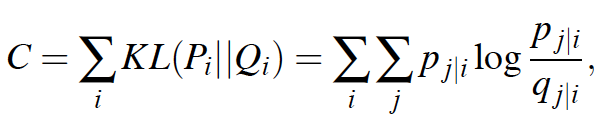
\includegraphics[scale=.3]{eq3}
% 	\caption{فرمول تابع $C$}\label{fig.eq3}
% \end{figure}
% \\
% در این فرمول $P_i$ به معنا‌ی توزیع شرطی احتمالی به روی تمام نقاط به غیر از $x_i$ می‌باشد و $Q_i$ نیز به معنای توزیع شرطی احتمالی به روی تمام نقاط نگاشت شده به غیر $y_i$ می‌باشد. به دلیل عدم تقارن تابع واگرایی کولبک-لایبلر، انواع مختلف خطا در فواصل دوتایی در داده‌های نگاشت شده‌ی کم بعد دارای وزن یکسانی نمی‌باشند. برای مثال، تابع هزینه بسیار افزایش پیدا می‌کند اگر دو داده‌ی دور از هم به دو داده‌ی نزدیک به هم نگاشت پیدا کنند اما تابع هزینه تغییر آنچنانی نمی‌کند اگر دو داده‌ی نزدیک به دو داده‌ی دور از هم نگاشت پیدا کنند.
% \\
% دلیل این اتفاق را می‌توان به این صورت بیان کرد که تابع هزینه اس ان ای تمرکز خود را بر روی حفظ ساختار محلی و انتقال آن به داده‌های نگاشت داده شده، قرار داده است.
% \\
% پارامتر واریانس ($\sigma_i$) نمی‌تواند برای تمام نقاط برابر باشد، برای مثال در مکان‌هایی با چگالی بالا مقدار واریانس کوچک بهتر عمل می‌کند. با افزایش پارامتر واریانس، آنتروپلی توزیع احتمال آن نقطه نیز افزایش پیدا می‌کند.
% \\
% روش اس ان ای برای پیدا کردن این مقدار،‌ از سرچ دودویی استفاده می‌کند و به دنبال مقداری از واریانس میگردد که توزیع احتمالی درست کند که سرگشتگی آن برابر با مقدار مشخص شده توسط کاربر باشد، سرگشتی طبق فرمول زیر تعریف می‌شود:
% \begin{figure}[!h]
% 	\centering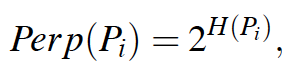
\includegraphics[scale=.3]{eq4}
% 	\caption{فرمول سرگشتگی}\label{fig.eq4}
% \end{figure}
% \\
% که در آن
% $H(P_i)$
% شانون آنتروپلی می‌باشد که فرمول آن به شکل زیر می‌باشد:
% \begin{figure}[!h]
% 	\centering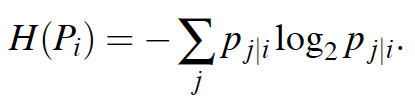
\includegraphics[scale=.3]{eq5}
% 	\caption{فرمول آنتروپی شنون}\label{fig.eq5}
% \end{figure}
% \\
% سرگشتگی می‌تواند به صورت اندازه‌گیری تعداد همسایه‌های موثر تفسیر شود.
% عملکر اس ان ای نسبت به تغییرات اندازه‌ی سرگشتی بسیار مقاوم است و مقادیر معمول این پارامتر، عددی بین ۵ تا ۵۰ می‌باشد.
% \\
% برای استفاده از روش شیب گرادیان برای کوچک کردن مقدار تابع $C$ از گرادیان این تابع استفاده می‌کنیم که فرمول آن به شکل زیر است:
% \begin{figure}[!h]
% 	\centering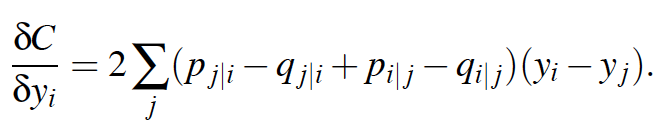
\includegraphics[scale=.3]{eq6}
% 	\caption{گرادیان تابع $C$}\label{fig.eq6}
% \end{figure}
% \\
% به صورت فیزیکی، گرادیان می‌تواند به صورت برآیند نیرو‌های فنرهایی بین نقطه‌ی نگاشت شده‌ی
% $y_i$
% و بقیه نقاط تفسیر شود، نیروی فنر بین دو داده‌ی
% $y_i$
% و داده‌ی
% $y_j$
% در راستای 
% $y_i-y_j$
% واقع شده است که این نیرو بر اساس میزان نزدیکی این دو داده در فضای اصلی با ابعاد بالا، می‌تواند به صورت جذبی یا دفعی باشد.
% \\
% نیروی هر فنر وابسته به طول آن (فاصله‌ی دو نقطه‌ی نگاشت شده) و سختی آن است که این سختی بر اساس فرمول 
% $(p_{j|i} - q_{j|i} + p_{i|j} - q_{i|j})$
% محاسبه می‌شود.
% \\
% روش شیب گرادیان کار خود را با سمپل کردن نقاط نگاشت پیدا شده به صورت اتفاقی از یک توزیع گوسی که حول مرکز واقع شده است شروع می‌کند. برای افزایش سرعت و همچنین پرهیز کردن از مینیمم‌های محلی، یک مقدار نسبتا بزرگ تکانه به گرادیان اضافه می‌شود، به عبارتی دیگر مقدار کنونی گرادین با مقادیر گرادیان‌های قبلی که به صورت تصاعدی و نزولی ضریب داده شده‌اند، جمع بسته می‌شود.
% به صورت کلی، فرمول بروز رسانی مقدار گرادیان به همراه تکانه به صورت زیر می‌باشد:
% \begin{figure}[!h]
% 	\centering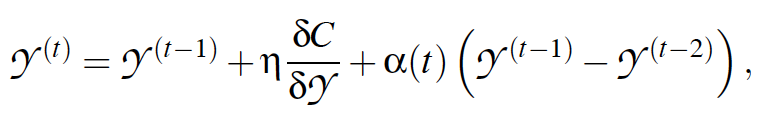
\includegraphics[scale=.3]{eq7}
% 	\caption{فرمول گرادیان به همراه تکانه}\label{fig.eq7}
% \end{figure}
% \\
% که در آن
% $\gamma^{(t)}$
% نماد نگاشت در مرحله‌ی $t$ام،
% $\eta$
% نماد ضریب یادگیری و
% $\aleph(t)$
% نماد تکانه در مرحله‌ی $t$ام می‌باشد.
% \\
% همچنین در مراحل اولیه الگوریتم، یک نویز گوسی به هر نقطه‌ی نگاشت شده، پس از هر مرحله اضافه می‌شود.
% کاهش به تدریج مقدار واریانس این نویز، باعث می‌شود که روش بتواند از مینیمم‌های محلی ضعیف،‌ فرار کند.
% در اس ان ای متاسفانه این روند نزول واریانس نویز و انتخاب مقدار اولیه آن، نیاز به تنظیم دستی توسط کاربر دارد و همچنین این مقادیر تاثیر زیادی بر روی خروجی خواهند داشت.
% \\
% همچنین پارمترهایی مانند تکانه و اندازه‌ی هر مرحله نیز نیاز به تنظیم دستی دارند.
% به همین دلیل به صورت معمول،‌ روش اس ان ای چندین بار بر روی داده با پارمتر‌های مختلف اجرا می‌شود و از بین آن‌ها خروجی بهتر انتخاب می‌شود.
% \\
% به طول کلی روش اس ان ای، نسبت به روش‌های دیگری که خروجی مناسبی را بدون نیاز به تنظیم دستی و زمان زیاد اجرای چند باره‌ی الگوریتم ارائه می‌دهند در سطح پایین‌تری قرار دارد.